\documentclass[11pt,a4paper]{article}

\usepackage{tpacdc}
\usepackage{hyperref}
\usepackage[normalem]{ ulem }
\usepackage{soul}
\usepackage{siunitx}
\usepackage{graphicx}
\usepackage{blindtext} % USE FOR LOREM IPSUM

% Custom colors
\usepackage{color}
\definecolor{deepblue}{rgb}{0,0,0.5}
\definecolor{deepred}{rgb}{0.6,0,0}
\definecolor{deepgreen}{rgb}{0,0.5,0}
\definecolor{gray}{rgb}{0.5,0.5,0.5}

\usepackage{listings}
\lstset{
  language=Python,
  basicstyle=\ttfamily\small,
  frame=single,
  numbers=left,
  keywordstyle=\color{deepblue},
  emphstyle=\color{deepred},
  stringstyle=\color{deepgreen},
  commentstyle=\color{gray},
  showstringspaces=false,
  keepspaces=true,
  inputencoding=utf8,
  extendedchars=true,
  literate={é}{{\'e}}1
           {°}{{\textdegree}}1,
  escapeinside={\%*}{*)}
}

\textheight 24cm
\textwidth 16cm
\oddsidemargin 0cm
\topmargin -0.5cm

\begin{document}
\enteteTPCS{0}{Septembre 2017}{TP C\#0: Nom Du TP}{1.0}

% Consignes de rendu
\section{introduction}
L'objectif de ce Workshop est de vous montrer quelques bases de
programmation dans un langage très simple pour débuter~: le Python.

Vous êtes encadrés par plusieurs étudiants et enseignants de l'EPITA. N'hésitez
pas à nous poser des questions !

Le but de ce Workshop est de vous faire dessiner des formes géométriques
à l'aide du langage de programmation
\emph{Python}\footnote{\url{http://python.org/}} et de son module
\emph{turtle}\footnote{\url{https://docs.python.org/3.6/library/turtle.html}},
un ensemble d'outils destinés aux débutants souhaitant découvrir la
programmation.  Vous trouverez en annexe des exemples de ce que vous serez
capable de réaliser avec ce module et les connaissances acquises au cours de ce
Workshop.

\section{L'environnement de développement}
\subsection{Généralités}

Dans un premier temps, regardons l'environnement qui sera utilisé pour réaliser
ce Workshop. Un environnement de développement est généralement composé de trois
outils~:

\begin{itemize}
    \item un éditeur~: l'espace éditable où vous taperez votre code~;
    \item un compilateur~: un logiciel qui traduira le code que vous aurez
        écrit afin qu'il soit compréhensible par l'ordinateur. Pour certains
        langages, ce compilateur est remplacé par un interpréteur (la différence
        n'a pas d'importance ici)~;
    \item un debugger~: un outil nous permettant d'analyser notre programme afin
        de corriger les erreurs qui s'y sont glissées.
\end{itemize}

Vous avez de la chance, il existe des logiciel qui combinent éditeur et
compilateur / interpréteur. On les appelle IDE (Integrated Development
Environnement - Environnement de développement intégré).

Nous utiliserons un IDE dédié à la programmation en Python~: PyScripter

\subsection{Votre IDE}

PyScripter se lance très simplement en double cliquant sur l'icône
associée se trouvant quelque part sur votre bureau. Si tout se passe
bien, vous devriez voir un écran similaire à celui de la figure~
\ref{fig:pyscripterstart}.

\begin{figure}
    \centering
    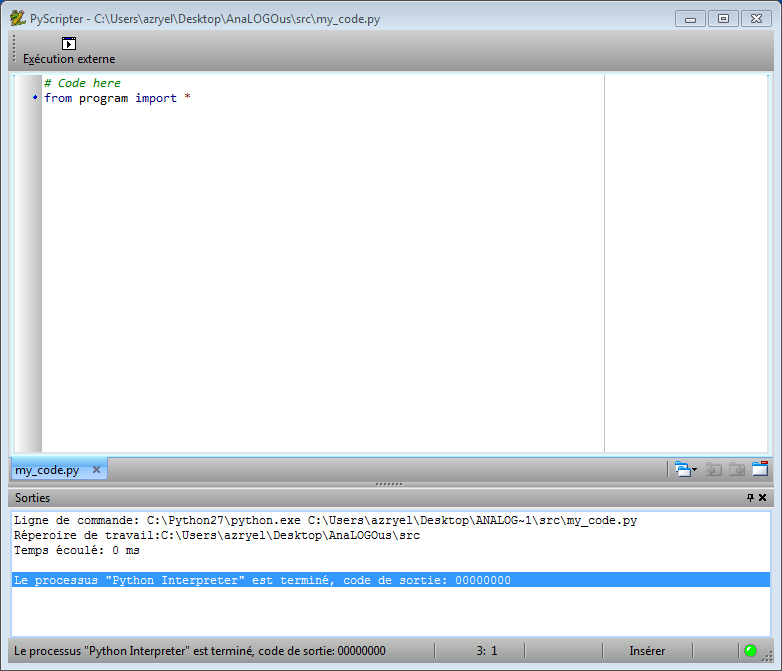
\includegraphics[width=0.8\textwidth]{img/capture}
    \caption{PyScripter après ouverture}
    \label{fig:pyscripterstart}
\end{figure}

Vous l'aurez compris, l'IDE n'affiche que le strict minimum nécessaire
pour ce Workshop. Notez que deux lignes de code sont déjà présentes~:

\begin{itemize}
    \item \lstinline{# Insérez votre code ici} est un commentaire, il sera ignoré par
        l'interpréteur, comme toutes les lignes commençant par \lstinline{#}.
    \item \lstinline{import turle} permet d'importer l'ensemble des fonctionnalités
        présentes dqns la bubliothèque turtle. Au niveau de l'interface de
        l'IDE, vous utiliserez principalement (de haut en bas)~;
    \item le bouton d'exécution~: presser ce bouton exécutera aussi votre code~;
    \item l'espace d'édition~;
    \item une console (onglet \emph{Sortie} en bas d'écran)~: c'est ici que
        s'afficheront les messages d'erreur si votre code n'est pas correct.
\end{itemize}

Si vous essayez d'exécuter le programme (en appuyant sur le bouton),
vous remarquerez qu'une fenêtre s'ouvre, et se ferme juste après. Votre
objectif sera de dessiner dans cette fenêtre~!

\newpage{}
\section{Premiers pas}

Pour l'instant, voyons ce qu'il est possible de faire avec quelques lignes de
code. Pour bien comprendre ce qu'il se passe~: recopiez dans votre fichier ce
qui est donné ici, changez les nombres, et voyez quelle œuvre d'art vous êtes en
train de créer~!

\subsection{Quelques primitives pour débuter}
Une première forme~:

\begin{lstlisting}
turtle.forward(100)
turtle.left(90)
turtle.forward(100)
turtle.left(90)
turtle.forward(100)
turtle.left(90)
turtle.forward(100)
\end{lstlisting}

Une autre~:

\begin{lstlisting}
turtle.forward(100)
turtle.left(120)
turtle.forward(100)
turtle.left(120)
turtle.forward(100)
\end{lstlisting}

\subsection{Éviter d'écrire les mêmes instructions~: les procédures}

Souvent, une forme géométrique est composée de plusieurs formes simples. Nous
pouvoins par exemple indiquer à l'ordinateur la procédure à suivre pour dessiner
ces formes simples. Cette procédure pourra ensuite être réutilisée plusieurs
fois afin de créer la forme plus complexe. En programmation, nous parlons de
\emph{procédure} ou \emph{fonction}. En réalité, vous aviez déjà rencontré cette
bestiole~: ce sont toutes les lignes que vous tapez et finissez par des
parenthèses. En effet, \lstinline{turtle.forward()}, \lstinline{turtle.left()},
etc. sont toutes des procédures cachant un code compliqué que vous appelez
plusieurs fois.

Le schéma général de déclaration de procédure est le suivant~:

\begin{lstlisting}
def nom_de_ma_super_procedure():    # on nomme la procedure
    instruction 1                   # tabulation obligatoire
    instruction 2
\end{lstlisting}

Prenez garde aux espaces avant chaque instruction~: cela permet au
compilateur/interpréteur de savoir que les instructions appartiennent
bien à la fonction\footnote{Certains langages ont une approche différente~: le
C, C++, Java, et C\# par exemple utilisent des accolades pour délimiter le corps
des fonctions. Les langages tels que Python ou encore le Haskell délimitent les
corps de fonctions par rapport à l'indentation, ce qui rend le code
\emph{naturellement} lisible.}.

Une fois définie, vous appelez votre procédure tout simplement comme
suit~:

\begin{lstlisting}
nom_de_ma_super_procedure()
\end{lstlisting}

\emph{Appeler} une procédure revient à exécuter le code qu'elle contient.

Voici quelques procédures que vous pouvez tester pour mieux comprendre :

\begin{figure}
    \centering
    
\includegraphics[width=0.8\textwidth]{img/square}
    \caption{\lstinline{carre()}}
    \label{fig:square}
\end{figure}

\begin{lstlisting}[float]
def carre():  # voir la figure %*\ref{fig:square}*)
    turtle.forward(100)
    turtle.left(90)
    turtle.forward(100)
    turtle.left(90)
    turtle.forward(100)
    turtle.left(90)
    turtle.forward(100)
\end{lstlisting}
\newpage

\begin{figure}
    \centering
    
\includegraphics[width=0.8\textwidth]{img/triangle}
    \caption{\lstinline{triangle()}}
    \label{fig:triangle}
\end{figure}

\begin{lstlisting}[float]
def triangle():  # voir la figure %*\ref{fig:triangle}*)
    turtle.forward(100)
    turtle.left(120)
    turtle.forward(100)
    turtle.left(120)
    turtle.forward(100)
\end{lstlisting}

\subsection{Créez vos propre procédures~!}

Il est maintenant temps de créer vos propres procédure. Essayez d'écrire des
procédure pour dessiner~:

\begin{itemize}
    \item une étoile~;
    \item un losange~;
    \item l'approximation d'un cercle (un cercle peut être approximé par une
        série de segments parcourant son bord). Vous pourrez utiliser les
        procédures \lstinline{math.cos(angle)} et \lstinline{math.sin(angle)}.
\end{itemize}

\begin{figure}
    \centering
    
\includegraphics[width=0.8\textwidth]{img/approx_circle}
    \caption{Exemple d'approximation de cercle}
    \label{fig:circle}
\end{figure}

\section{Répéter plusieurs fois les mêmes opérations~: les boucles}

En général, on parviendra à dessiner une forme complexe avec un certain nombre
de formes simples.

En fait, jusqu'à présent, vous dessiniez déjà des formes relativement complexes
à partir d'une autre plus simple~: la ligne.

En observant bien, pour dessiner un carré, on exécute quatre fois les mêmes
instructions~:

\begin{lstlisting}
# on dessine un bord
turtle.forward(100)
# on tourne de 90° : la direction du second bord
turtle.right(90)
# et on recommence
turtle.forward(100)
turtle.right(90)
turtle.forward(100)
turtle.right(90)
turtle.forward(100)
turtle.right(90)
# les quatre bords apparaissent
\end{lstlisting}

Pour faire plus court, il serait intéressant de pouvoir dire à
l'ordinateur :

\begin{lstlisting}
faire 4 fois :
    avancer de 100 points
    tourner de 90°
\end{lstlisting}

Il s'avère que cela est possible en Python. C'est ce que l'on appelle une
\emph{boucle}. Dans le cas du carré, on obtient en Python\footnote{Remarquez
l'usage de la procédure \lstinline{range(nombre)}. Elle génèrera une suite de
nombres allant de \lstinline{0} à \lstinline{nombre - 1.}}~:

\begin{lstlisting}
for i in range(4):     # faire 4 fois :
    turtle.forward(100)     # avancer de 100 points
    turtle.right(90)        # tourner de 90°
\end{lstlisting}

Maintenant réécrivez toutes les formes que vous avez déjà programmées, mais en
utilisant les boucles~:

\begin{itemize}
\item le triangle~: en 3 lignes de code~;
\item le losange~: en 3 ligne de codes~;
\item l'approximation de cercle~: en 3 ligne de codes.
\end{itemize}

\section{Quelques objectifs simples}
Cette fois ci, vous n'êtes plus guidés~! Montrez que vous êtes créatifs en
réussissant à dessiner les formes suivantes avec le moins de ligne de code
possible. N'hésitez pas à appeler à l'aide~!

\begin{figure}[H]
    \centering
    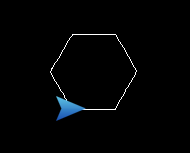
\includegraphics[height=0.4\textwidth]{img/approx_circle_hexagon}
    
\includegraphics[height=0.4\textwidth]{img/star}
    \caption{Autres exemples de forme géométriques}
    \label{fig:ending_examples}
\end{figure}

\section{Quelques objectifs impossibles}

Les dessins suivants sont bien plus difficiles à réaliser que les autres~!
Certains nécessitent même des notions bien plus complexes que celles vues dans
ce TP~: saut conditionnel, récursion, passage de paramètre aux procédures, etc.

Nous mettons à votre disposition d'autres procédures pour permettre à
votre créativité de mieux s'exprimer~:

\begin{itemize}
    \item \lstinline{turtle.speed(vitesse)}~: change la vitesse de tracé du dessin, pour
        aller le plus vite possible, choisissez \lstinline{0}.
    \item \lstinline{turtle.penup()}~: les prochains déplacement n'afficheront rien~;
    \item \lstinline{turtle.pendown()}~: a l'effet inverse du lever de crayon~;
    \item \lstinline{turtle.pensize(taille)}~: change la taille des prochains traits
        dessinés~;
    \item \lstinline{turtle.pencolor(rouge, vert, bleu)}~: change la couleur des
        prochains traits dessinés. Notez que les couleurs ont trois
        composantes~: vert, rouge et bleu. Chacune peut avoir une valeur allant
        de 0 (absence de la composante) à 1. Par exemple, du rouge pur
        correspond à la combinaisons \lstinline{(rouge = 1, vert = 0, bleu = 0)}
        et le gris à \\ \lstinline{(rouge = 0.5, vert = 0.5, = bleu = 0.5)}.
\end{itemize}

Essayez d'obtenir le bon résultat, et appelez un assistant dès que vous
bloquez~!

\begin{figure}[H]
    \centering
    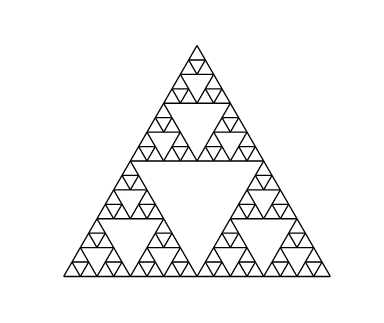
\includegraphics[width=0.8\textwidth]{img/sierpinski}
    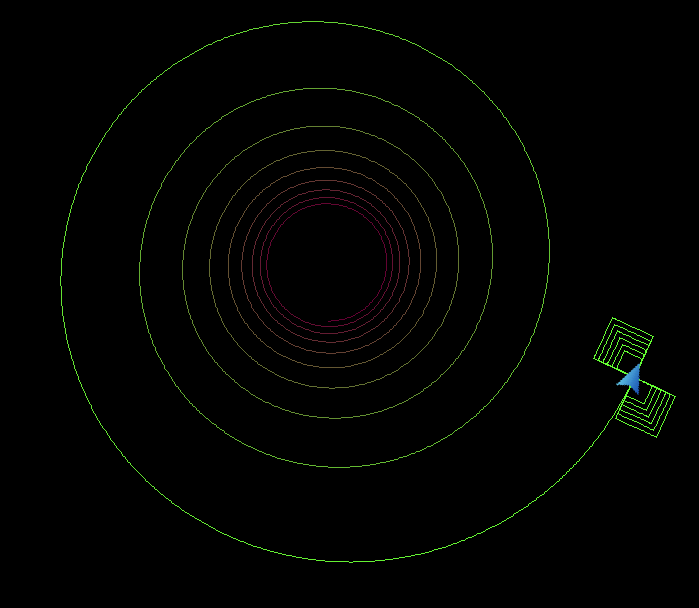
\includegraphics[width=0.8\textwidth]{img/spiral_square}
    \caption{Exemples de fractales}
    \label{fig:fractales}
\end{figure}

\end{document}
